\documentclass[runningheads]{llncs}
\usepackage[T1]{fontenc}
\usepackage{graphicx}
\usepackage{amsmath} 
\begin{document}

\title{Creation of a Pseudodictionary to Minimize the Ambiguity}

\graphicspath{{images/}}

\author{Luca Barra}


\institute{
  Department of Computer Science, University of Turin, Turin, Italy \\
  \email{luca.barra@edu.unito.it}
}

\maketitle

\begin{abstract}
This paper investigates the construction of cross-lingual pseudodictionaries designed to minimize lexical ambiguity through optimal translation pair selection. Building on the observation that historical, cultural, and geographic factors create varying degrees of sense alignment between languages, I propose a method that systematically selects word pairs ($L_1$-$L_k$) maximizing the Ambiguity Reduction Score (ARS). My approach leverages these naturally occurring asymmetries in semantic overlap to create a resource that preferentially includes translation pairs demonstrating the strongest sense alignment. The resulting pseudodictionary provides empirically optimized word mappings that significantly reduce polysemy. It has applications in machine translation and word sense disambiguation.
\keywords{NLP \and Languages \and Semantic.}
\end{abstract}

\section{Introduction}

\subsection{The Key Idea}

Consider a word $x \in L_1$ with $N$ senses and its translation $y \in L_2$ with $M$ senses (where $M \leq N$). We can bind $x$ to $y$ to create a new lexical unit called \textit{pseudoword}, denoted $x-y$. This new unit $x-y$ inherits only the common senses between the two starting word resulting in a word that is less ambiguous than either $x$ or $y$ individually. Formally:

\begin{itemize}
  \item Let $\mathcal{S}_x$ be the set of senses of $x$ in $L_1$
  \item Let $\mathcal{S}_y$ be the set of senses of $y$ in $L_2$
  \item The senses of the pseudoword $x \cdot y$ are $\mathcal{S}_{x \cdot y} = \mathcal{S}_x \cap \mathcal{S}_y$
\end{itemize}

\[
  |\mathcal{S}_{x-y}| \leq \text{min}(|\mathcal{S}_x|, |\mathcal{S}_y|)
\]

In particular, it frequently holds that:
\[
|\mathcal{S}_{x \cdot y}| \ll |\mathcal{S}_x| \quad \text{and} \quad |\mathcal{S}_{x \cdot y}| \ll |\mathcal{S}_y|
\]

\subsection{Ambiguity Reduction Score (ARS)}

A simple approach to measure the reduction of ambiguity of a pseudoword $x-y$ is to use a score like: 

\[
  \text{AmbiguityReduction}(x, y) = \frac{|\mathcal{S}_x| + |\mathcal{S}_y| - 2 \cdot |\mathcal{S}_x \cap \mathcal{S}_y|}{|\mathcal{S}_x| + |\mathcal{S}_y|}
\]

where $|\mathcal{S}_x|$ is the set of sense in $x$, $|\mathcal{S}_y|$ is the set of sense in $y$ and $|\mathcal{S}_{x-y}$ is the set of common sense between $x$ and $y$. Taking a step further we can generalize the formula to take $N$ languages: 


\[
  \text{AmbiguityReduction} = \frac{\sum_{i=1}^N |\mathcal{S}_i| - N \cdot \left|\bigcap_{i=1}^N \mathcal{S}_i\right|}{\sum_{i=1}^N |\mathcal{S}_i|}
\]

where $|\bigcap_{i=1}^N \mathcal{S}_i| \cdot N$ are the sense shared in all the languages and $\sum_{i=1}^N |\mathcal{S}_i|$ are the total number of sense across all the languages.

This score ranges between 0 and 1:
\begin{itemize}
  \item A score of 0 ($N \cdot \left|\bigcap_{i=1}^N \mathcal{S}_i\right| \rightarrow 1$) indicates no reduction in ambiguity, all languages share exactly the same set of senses.
  \item A score close to 1 ($N \cdot \left|\bigcap_{i=1}^N \mathcal{S}_i\right| \rightarrow 0$) indicates maximum disambiguation, there is little or no overlap between the senses of words across languages.
\end{itemize}

\section{The Pseudodictionary}

\subsection{The Ambiguity between Different Languages}

The foundational hypothesis of this work posits that lexical compatibility between languages operates at the word-level rather than being a language-wide property. This manifests as significant variance in ARS potential between specific word pairs across different languages:

\begin{itemize}
  \item The word form "Fiore" (IT) and the word form "Blume" (DE) have an ARS greater than "Fiore" and "Flower" (EN). 
  \item The word form "Carne" (IT) and the word form "Meat" (EN) have an ARS Score greater than "Carne" and "Fleish"(DE). 
\end{itemize}

We can use this fact to construct a pseudodictionary that contains only pairs of words with the maximum ARS. This can be done with the following passage: 
\begin{itemize}
  \item Let $w \in L_1$.
\item For each language $L_j \in {L_2,\ldots,L_n}$:
\begin{itemize}
\item Retrieve all potential translations $T_j = {t_{j1},\ldots,t_{jk}}$ in $L_j$.
\item For each translation candidate $t_{ji} \in T_j$:
\begin{itemize}
  \item Extract all senses from $w$ and $t_{ji}$.
\item Compute ARS for each pair.
\item Record the maximal ARS for this word pair.
\end{itemize}
\end{itemize}
\item Identify the optimal pair $(w, t_{ji})$ that achieves the highest ARS across all languages.
\end{itemize}
\subsection{How to Choose a Translation}

A key challenge in this approach is selecting optimal translations. A potential approach is to:
\begin{itemize}
\item Evaluate all possible translations of $x$ across target languages.
\item Select the pairing that maximizes the ARS (tab. \ref{tab1}).
\end{itemize}

The major advantage of this selection process is that it produces the \textit{least ambiguous pseudoword} possible from the combination $L_1$–$L_2$. This in turn enables the possibility of comparisons across other pseudowords in different language pairs (e.g., $L_1$–$L_3$, $L_1$–$L_4$, etc.) with uniformly reduced ambiguity.

\begin{table}[ht]
\centering
\caption{Example with some translation (EN-IT). The pseudoword Room-Camera is better than the pseudoword Room-Chamber.}\label{tab1}
\begin{tabular}{|l|l|l|c|}
\hline
Word $L_1$ & Translation $L_2$ & Common Senses & ARS \\
\hline
Room & Camera & 
\begin{tabular}[t]{@{}l@{}}
Room (Architecture) \\ 
Room (Novel) \\
The Room (2003) \\
The Room (2015)
\end{tabular} & 0.500 \\
\hline
Chamber & Camera & 
\begin{tabular}[t]{@{}l@{}}
Chamber (firearms) \\
Bedroom \\
Room \\
Legislative chamber \\
Chambers (law) \\
Room (Architecture) \\
The Chamber (Song) \\
The Chamber (1996)
\end{tabular} & 0.176 \\
\hline
\end{tabular}
\end{table}

This is only one of the possible approach:

\begin{itemize}
  \item \textbf{Backward-Translation}: 
    \begin{itemize}
      \item Translate the source word $x \in L_1$ into the target language $L_2$, yielding a candidate translation $t_x \in L_2$.
      \item Then, translate $t_x$ back from $L_2$ into the source language $L_1$, obtaining $y \in L_1$.
      \item If the back-translated word $y$ matches the original word $x$ (i.e., $x = y$), then $t_x$ is considered a valid translation and can be selected.
      \item If no candidate satisfies this condition, or if multiple candidates yield the same back-translation, fall back to an alternative selection strategy.
    \end{itemize}
  \item \textbf{Combining Multiple Technique}: as show by Hyun Lee, Juntae Yoon and Gil-Chang Kim \cite{Translation2003}, it is possible to combine different measures:

\begin{itemize}
  \item \textbf{Sense preference:} leverages example sentences and glosses from a bilingual dictionary to identify the most probable sense of a word in context.

  \item \textbf{Sense probability:} Uses bilingual dictionaries to map each source sense to a distinct set of target words. These clusters are typically semantically coherent. By selecting the cluster with the highest contextual fit (via co-occurrence statistics), we reduce the chance of including semantically divergent or spurious translations.

  \item \textbf{Word probability:} Once a sense is selected, target words within the same sense cluster are ranked by their naturalness in context, measured via co-occurrence frequency in a corpus. This ensures the final translation minimizes lexical ambiguity and aligns with native usage.
\end{itemize}
\end{itemize}

\section{Experiments and Results}

The method was tested using selected words\footnote{For computational simplicity, the problem of selecting the optimal translation was omitted, and only the most common translations were considered.} in Italian ($L_1$), English ($L_2$), and German ($L_3$). As shown in Figure \ref{fig:1}, pseudowords like \textit{pesca-pfirsich} and \textit{flower-blume} achieve a higher ARS than their counterparts in Figure \ref{fig:2}. However, certain pseudowords in Figure \ref{fig:2}, such as \textit{testa-head}, demonstrate a higher ARS than their alternatives.

\begin{figure}[!h]
    \centering
    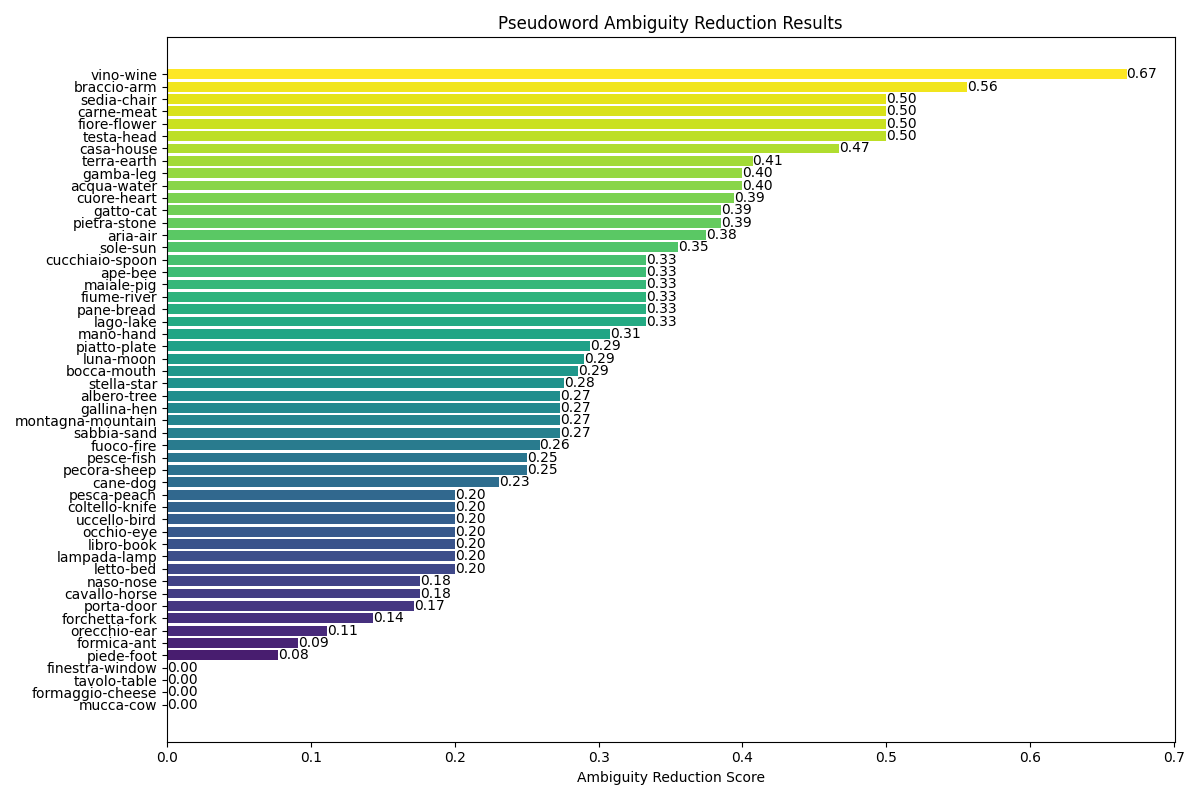
\includegraphics[scale=0.45]{ambiguity_reduction_plot_IT_EN.png}
    \caption{Ambiguity Reduction Score for IT-EN.}
    \label{fig:1}
\end{figure}
\begin{figure}[!h]
    \centering
    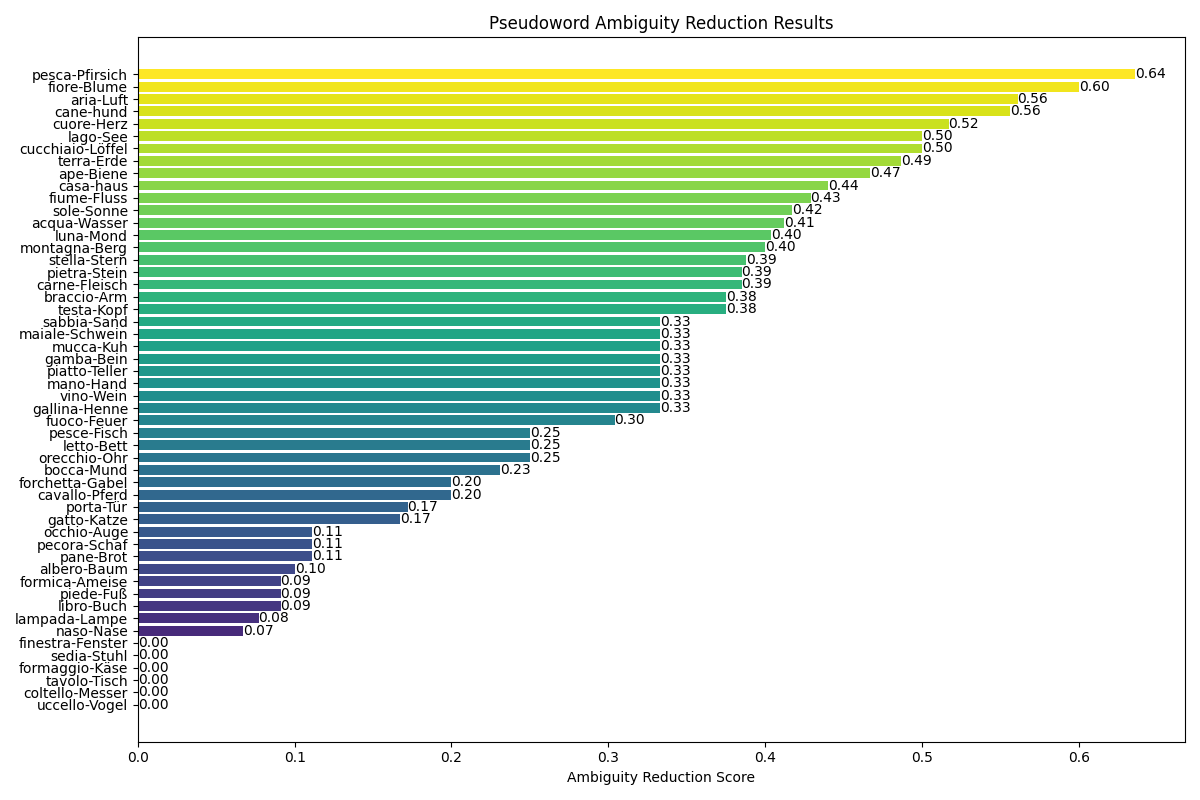
\includegraphics[scale=0.45]{ambiguity_reduction_plot_IT_DE.png}
    \caption{Ambiguity Reduction Score for IT-DE.}
    \label{fig:2}
\end{figure}


\subsection{Limitations}

A significant limitation of this approach stems from the scarcity of comprehensive multilingual semantic resources. Even when using BabelNet \cite{BabelNet2012}, one of the most extensive multilingual encyclopedias, several challenges persist:

\begin{itemize}
\item \textbf{Asymmetrical sense alignment}: Semantic mappings frequently operate unidirectionally (e.g., Italian $\rightarrow$ English mappings differ from English $\rightarrow$ Italian). This is demonstrated when querying with EN as \texttt{searchLang} and IT as \texttt{targetLang} produces different results than the reverse configuration.
\item \textbf{Sense noise from multiple sources}: BabelNet aggregates senses from diverse resources (e.g., WordNet, Wikipedia, OmegaWiki), resulting in redundancy. For instance, the word \textit{apple} has overlapping but differently phrased senses like "Fruit with red or yellow or green skin..." (WordNet) and "An apple is a round, edible fruit..." (Wikipedia). To reduce this noise, I restricted sense extraction to a single source (Wikipedia), improving consistency but at the cost of potentially losing valid senses from other sources.
\item \textbf{Incomplete coverage}: Many words lack proper cross-lingual sense mappings.
\item \textbf{Under-representation}: Low-resource languages are poorly represented in semantic networks, limiting the quality and size of pseudodictionaries involving those languages.
\end{itemize}


\section{Future Prospect}

\begin{itemize}
\item \textbf{Multilingual Scaling}: If a word $x \in L_1$ is combined with a word $y \in L_2$, the resulting pseudoword $x-y$ is less ambiguous than the original words. Naturally, adding a word $z \in L_3$ would further reduce ambiguity (as demonstrated by the generalized ARS formula). The key challenge lies in identifying the optimal combination of languages that maximizes the ARS, thereby achieving the greatest ambiguity reduction.
  \item \textbf{Pseudodictionary as a Semantic Benchmark}: The constructed pseudodictionary could be evaluated as a benchmark for word sense disambiguation (WSD) systems. Since pseudowords inherently have reduced ambiguity, they provide a controlled environment for assessing semantic alignment algorithms across languages.
\item \textbf{Machine Translation}: The pseudodictionary increases machine translation performance by reducing polysemy, enabling models to learn clearer, sense-specific mappings that minimize mistranslations and improve lexical precision.
\end{itemize}

\begin{thebibliography}{8}
\bibitem{BabelNet2012}
Navigli, R., Ponzetto, S.P.: BabelNet: The Automatic Construction, Evaluation and Application of a Wide-Coverage Multilingual Semantic Network. Artificial Intelligence 193, 217--250 (2012). \url{https://doi.org/10.1016/j.artint.2012.07.001}
\bibitem{Translation2003}
Lee Hyun, Yoon Juntae, Kim Gil-Chang. (2003). Translation Selection by Combining Multiple Measures for Sense Disambiguation and Word Selection. Int. J. Comput. Proc. Oriental Lang.. 16. 219-239. \url{https://doi.org/10.1142/S0219427903000905}. 
\end{thebibliography}

\end{document}
